\documentclass{article}
\usepackage{cite}
\usepackage{graphicx}
\usepackage{subcaption}
\usepackage{amssymb}
\usepackage{mathtools}
\usepackage{blindtext}
\usepackage{caption}
\usepackage[a4paper]{geometry}
\geometry{top=2.5cm, bottom=2.5cm, left=2.5cm, right=2.5cm}
\usepackage{fancyhdr}
\pagestyle{fancy}
\usepackage{hyperref}
\hypersetup{colorlinks=true,urlcolor=blue}
\usepackage{wrapfig}

\fancyhead[LO,RE]{Mètodes numèrics II}
\fancyhead[RO,LE]{PRÀCTICA 1}

\graphicspath{ {images/} }

\begin{document}
\thispagestyle{empty}
\begin{center}
    {\LARGE \textsc{Pràctica 1: Modelització del tractament}}\\ 
    \vspace{0.2cm}
    {\LARGE \textsc{d'ablació cardíaca IVS}}\\ 
    \vspace{0.2cm}
    $\begin{matrix} 
    \text{Miguel A.} \hspace{1.5cm} & \text{Daniel G.} & \hspace{1.5cm} \text{Gerard B.}\\1637738 \hspace{1.5cm} & 1666471 & \hspace{1.5cm} 1670235
    \end{matrix}$

    
\end{center}
\section{Introducció i problema}
Una ablació cardíaca IVS és una cirugia simple que s'aplica a pacients que pateixen arritmies i que reaccionen negativament a tractaments amb fàrmacs. De forma simplificada, aquesta intervenció consisteix en introduïr electrodes de polaritat oposada i local·litzar-los al cor sobre el teixit malalt. L'objectiu és fer servir l'efecte Joule per a escalfar el teixit malalt i provocar-ne la mort cel·lular de forma local. A l'hora d'aplicar aquest procediment quirúrgic cal tenir en compte algunes precaucions. La regió de teixit malalt ha d'estar entre els \(50\,\text{ºC}\) i \(80\,\text{ºC}\), la regió sana no ha de superar els \(50\,\text{ºC}\) i cap regió ha de sobrepassar els \(80\,\text{ºC}\).\\\\
A aquesta pràctica intentarem modelitzar aquest procediment realitzant diferents aproximacions i tenint en compte algunes restriccions. Trobarem una solució analítica al problema i la commpararem amb diverses solucions numèriques simulades amb Fortran.\\\\
Per a modelitzar el problema farem servir la llei de Fourier per a la temperatura:
\begin{equation*}
    c_{v}\rho \frac{\partial T}{\partial t} = \nabla (\kappa \nabla T) + P_{\text{ext}}
\end{equation*}
on $c_{v}$ és la calor específica, $\rho$ és la densitat, $\kappa$ és la conductivitat tèrmica i $P_{\text{ext}}$ fa referència a totes les fonts de calor externes del sistema. El model simplificat que farem servir serà in condensador planoparal·lel format per dos superfícies circulars que defineixen un volum cilíndric on hi ha teixit sa i teixit malalt al centre. Per aplicar més simplificacions al problema, asumirem que aquest teixit malalt també ocupa un volum cilíndric (veure Figura \ref{esquema_model}). 

\begin{figure}[h]
    \centering
    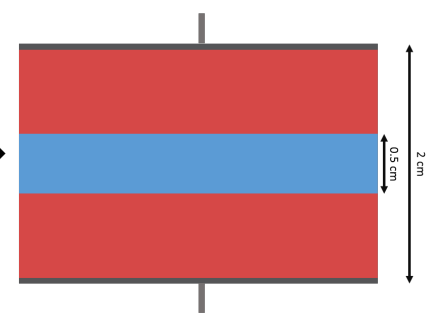
\includegraphics[width = 0.4\linewidth]{images/esquema_temp.png}
\end{figure}

Com a condicions inicials i de frontera tindrem en compte la temperatura del cos humà: \(T_c = 36.5\,\text{ºC}\). Aquesta temperatura ha de manternir-se sempre constant ja que el flux de sang provinent de la resta del cos no para en cap moment.
\section{Equació problema i adimensionalització}
A partir de la llei de d'Ohm podem trobar l'aportació externa de calor obtinguda per efecte Joule:
\begin{equation*}
    \vec{J} = \sigma\vec{E} \hspace{0.3cm} \Rightarrow \hspace{0.3cm} P_{\text{ext}} = \vec{J}\cdot\vec{E} = \sigma E^2 = \frac{\sigma}{2} \frac{(\Delta \phi)^2}{D^2}
\end{equation*}
on $\sigma$ és la conductivitat elèctrica del teixit i $D$ i $\Delta \phi$ son la distància i la diferència de potencial elèctric entre els electrodes, respectivament. Aprofitant la simetria cilíndrica del model, podem escriure la llei de Fourier com
\begin{equation*}
    c_{v}\rho \frac{\partial T}{\partial t} = \kappa \frac{\partial ^2 T}{\partial z^2} + \frac{\sigma}{2} \frac{(\Delta \phi)^2}{D^2}
\end{equation*}
A partir de definir
\begin{equation*}
    T = T_c \tilde{T} \hspace{0.3cm} \text{,} \hspace{0.3cm} t = \frac{T_c \kappa}{\alpha P_{\text{ext}}}\tilde{t} \hspace{0.3cm} \text{,} \hspace{0.3cm} z = \sqrt{\frac{T_c \kappa}{P_{\text{ext}}}}\tilde{z}
\end{equation*}
Trobem l'equació normalitzada que farem servir per a resoldre el nostre problema:
\begin{equation}\label{EDP_norm}
    \frac{\partial \tilde{T}}{\partial \tilde{t}} = \frac{\partial ^2 \tilde{T}}{\partial \tilde{z}^2} + 1 
\end{equation}
\section{Solució analítica de la EDP}
Com hem dit, els següents apartats els dedicarem a resoldre l'equació diferencial en derivades parcials \eqref{EDP_norm}. Notem que aquesta equació té solució analítica. Al resoldre l'equació seguint el procediment que s'observa a l'Annex \ref{Annex I} obtenim la següent solució normalitzada:
\begin{equation*}
    \tilde{T}(x,t) = T_c + \sum_{i=0}^{\infty} \frac{ 1-e^{-(2n+1)^2 \pi^2 \tilde{t}}}{(2n+1)^3\pi^3}\cdot 4\sin((2n+1)\pi \tilde{z})
\end{equation*}

\section{Solucions numèriques}
\subsection{Euler Explícit}
Discretitzant la derivada temporal per la dreta obtenim la relació de recurrència:
\begin{equation*}
    \tilde{T}_{j}^{i+1} = \gamma (\tilde{T}_{j+1}^{i}-2\tilde{T}_{j}^{i}+\tilde{T}_{j-1}^{i}) + \tilde{T}_{j}^{i} + \Delta \tilde{t}
\end{equation*}
on definim $gamma = \Delta \tilde{t}/(\Delta \tilde{z})^2$ Diferents valors de $\gamma$ ens porten a diferents mallats i pot influir a l'estabilitat dels diferents mètodes numèrics que podem aplicar.\\\\
Fem servir el mètode d'Euler Explícit \cite{Navau2024} amb diversos mallats per trobar la distribució de temperatures en $\tilde{t}=0.025$. En la Fig. \ref{fig:euler_explicit} i Fig. \ref{fig:err_euler_explicit} s'exposen les gràfiques $\tilde{T}$ vs $\tilde{z}$ i les comparacions de l'error per a cada mallat. El resultat amb el mallat $0.51$ i es pot observar com la solució oscil·la en forma de "dents de serra". Això és la inestabilitat numèrica degut a la simplesa del mètode i fer servir un pas temporal massa gran.  En la Fig. \ref{fig:euler_exp_at1} i Fig. \ref{fig:euler_exp_at2} s'exposa el resultat pel mallat de $0.49$ i $0.25$. Notem que per mallats menors a $0.5$ desapareixen les fluctuacions i la solució de l'equació de difusió es fa estable.

\begin{figure}[h]
    \centering
    \begin{subfigure}[b]{0.32\textwidth}
        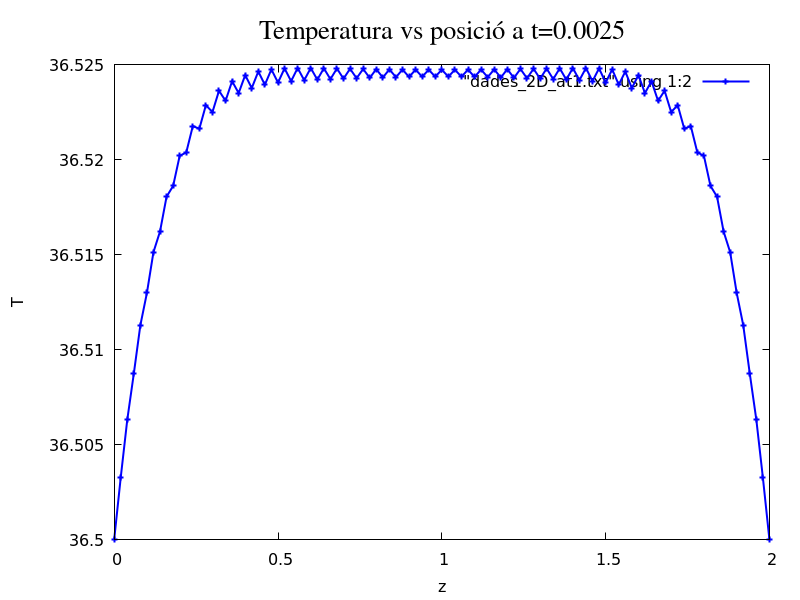
\includegraphics[width=\textwidth]{images/T_vs_z_at1.png} 
        \caption{}
        \label{fig:euler_exp_at1}
    \end{subfigure}
    \hfill
    \begin{subfigure}[b]{0.32\textwidth}
        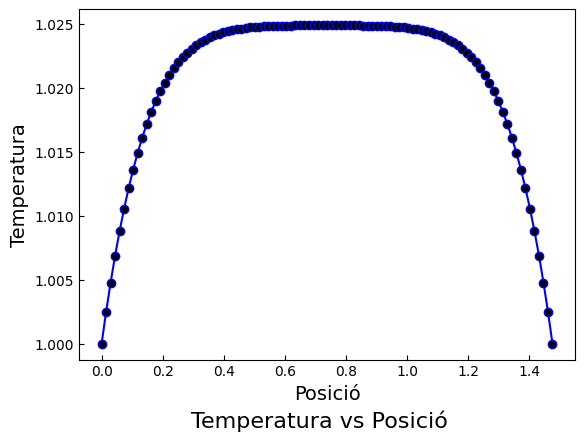
\includegraphics[width=\textwidth]{images/T_vs_z_at2.png}
        \caption{} 
        \label{fig:euler_exp_at2}
    \end{subfigure}
    \hfill
    \begin{subfigure}[b]{0.32\textwidth}
        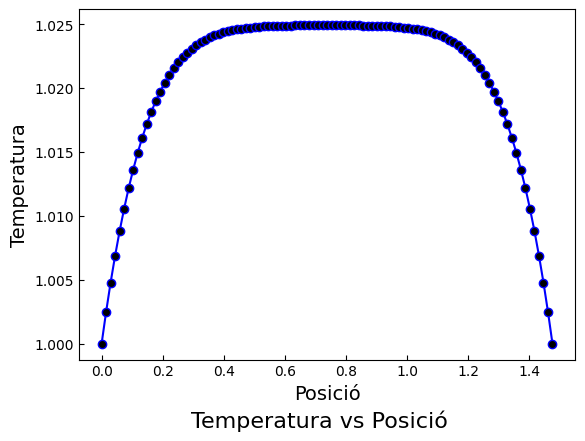
\includegraphics[width=\textwidth]{images/T_vs_z_at3.png}
        \caption{} 
        \label{fig:euler_exp_at2}
    \end{subfigure}
    \caption{Solució numèrica pel mallat 0.51 (a), 0.49 (b) i 0.25 (c) a $t=0.025$ fent servir el mètode d'Euler explícit.}
    \label{fig:euler_explicit}
\end{figure}
\begin{figure}[h]
    \centering
    \begin{subfigure}[b]{0.32\textwidth}
        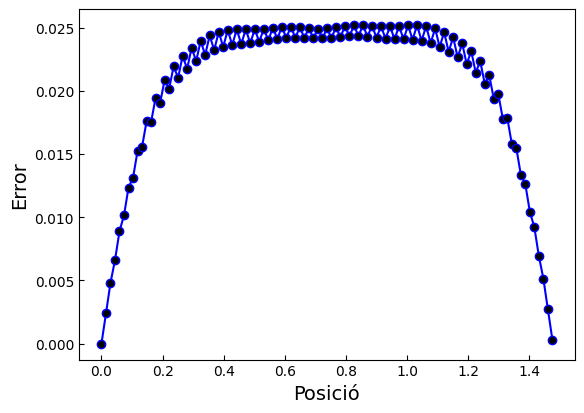
\includegraphics[width=\textwidth]{images/Error_vs_pos_at1.png} 
        \caption{}
        \label{fig:err_euler_exp_at1}
    \end{subfigure}
    \hfill
    \begin{subfigure}[b]{0.32\textwidth}
        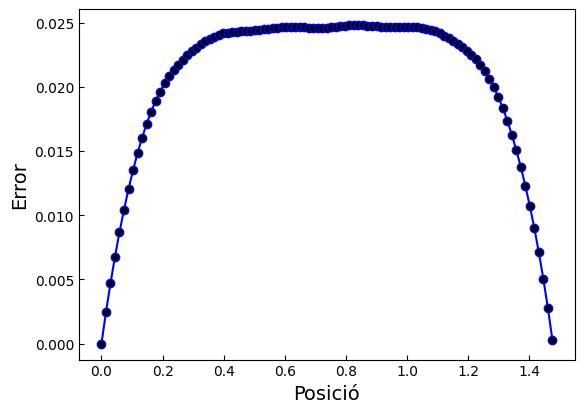
\includegraphics[width=\textwidth]{images/Error_vs_pos_at2.png}
        \caption{} 
        \label{fig:err_euler_exp_at2}
    \end{subfigure}
    \hfill
    \begin{subfigure}[b]{0.32\textwidth}
        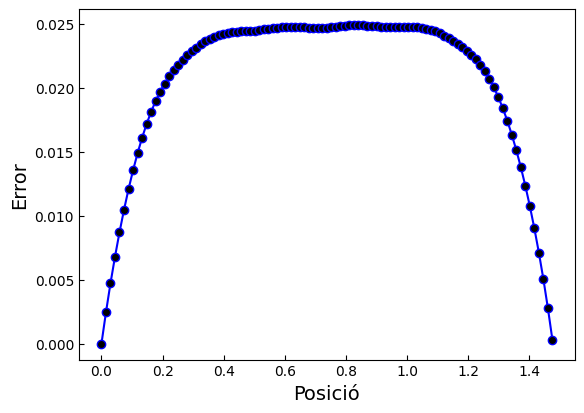
\includegraphics[width=\textwidth]{images/Error_vs_pos_at3.png}
        \caption{} 
        \label{fig:err_euler_exp_at2}
    \end{subfigure}
    \caption{Error numèric del mètode d'Euler explícit respecte la solució analítica per al mallat 0.51 (a), 0.49 (b) i 0.25 (c) a $\tilde{t}=0.025$}
    \label{fig:err_euler_explicit}
\end{figure}

\subsection{Euler Implícit}
Fem servir el mètode d'Euler implícit per a resoldre l'equació normalitzada \eqref{EDP_norm}. Discretitzant la derivada temporal per l'esquerra arribem a la següent expressió
\begin{equation}\label{disc_eu_imp}
    \tilde{T}_{j}^{i-1} = -\gamma \tilde{T}_{j+1}^{i} + (1+2\gamma)\tilde{T}_{j}^{i} - \gamma\tilde{T}_{j-1}^{i} - \Delta t
\end{equation}
Podem reescriure aquesta expressio en forma matricial
\begin{equation*}
    \vec{T}_{i-1} = \mathbb{M}\vec{T}_{i} + \vec{b}
\end{equation*}
on aïllem el terme $\vec{T}_i$ per a poder iterar i on definim
\begin{equation*}
    \vec{T}_{i} = \begin{matrix} ( \tilde{T}_{2}^{i} & \dots & \tilde{T}_{N-1}^{i} )^{\text{t}} \end{matrix} \hspace{4 mm} \text{,} \hspace{4 mm} \vec{b} = \begin{matrix} ( -(T_c + \Delta t) & -\Delta t &\dots&-\Delta t & -(T_c + \Delta t) )^{\text{t}} \end{matrix} 
\end{equation*}
\begin{equation*}
    \mathbb{M} = \text{tridiag}(-\gamma,1+2\gamma,-\gamma)
\end{equation*}
és a dir, el vector $\vec{T}_{i}$ emmagatzema tots els punts espaials de $\tilde{T}$ al temps $i$ sense tenir en compte les condicions de contorn. Aquestes es troben de forma implícita al vector $\vec{b}$. La matriu $\mathbb{M}$ és una matriu tridiagonal, on segons aquesta notació la diagonal inferior correspon a la primera entrada $-\gamma$, la diagonal principal a la segona entrada $(1+2\gamma)$ i la tercera entrada a la diagonal superior, $-\gamma$.\\\\
Fent les iteracions corresponents obtenim les figures que s'observen a la Fig. \ref{fig:euler_implicit} i Fig. \ref{fig:err_euler_implicit}.
\begin{figure}[h]
    \centering
    \begin{subfigure}[b]{0.35\textwidth}
        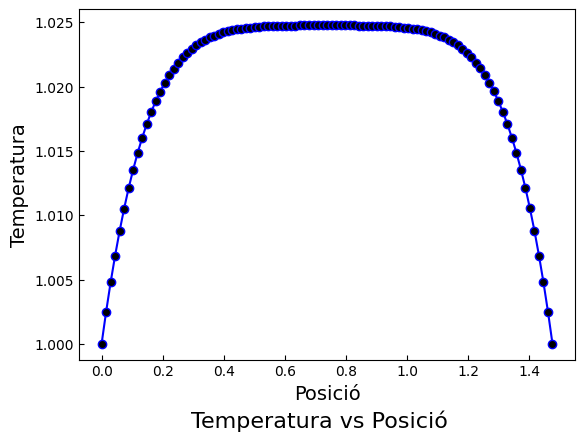
\includegraphics[width=\textwidth]{images/T_vs_z_imp_at1.png} 
        \caption{}
        \label{fig:euler_imp_at1}
    \end{subfigure}
    \hspace{1.5cm}
    \begin{subfigure}[b]{0.35\textwidth}
        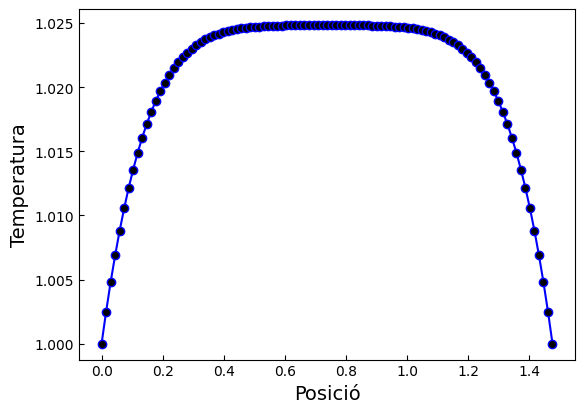
\includegraphics[width=\textwidth]{images/T_vs_z_imp_at2.png}
        \caption{} 
        \label{fig:euler_imp_at2}
    \end{subfigure}
    \caption{Solució numèrica pel mallat 1.0 (a) i 0.5 (b) a $\tilde{t}=0.025$ fent servir el mètode d'Euler implícit.}
    \label{fig:euler_implicit}
\end{figure}
\begin{figure}[h]
    \centering
    \begin{subfigure}[b]{0.35\textwidth}
        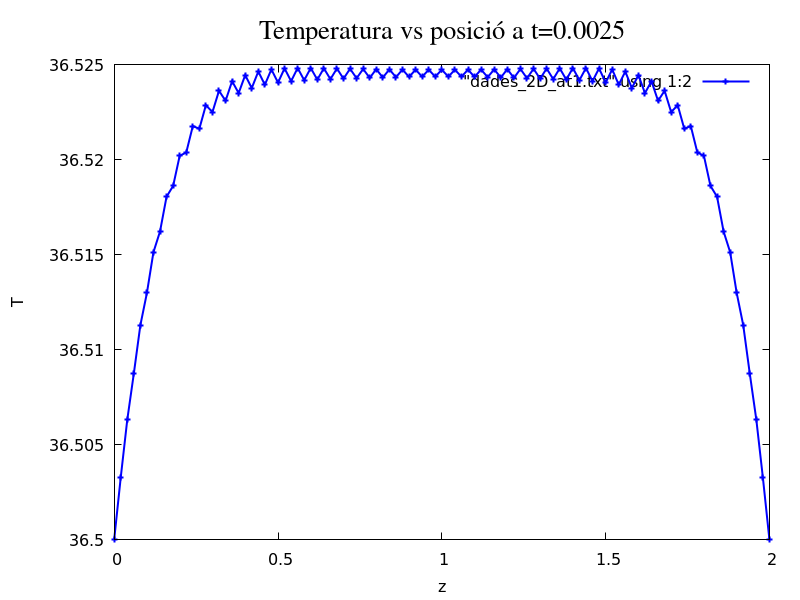
\includegraphics[width=\textwidth]{images/T_vs_z_at1.png} 
        \caption{}
        \label{fig:err_euler_imp_at1}
    \end{subfigure}
    \hspace{1.5cm}
    \begin{subfigure}[b]{0.35\textwidth}
        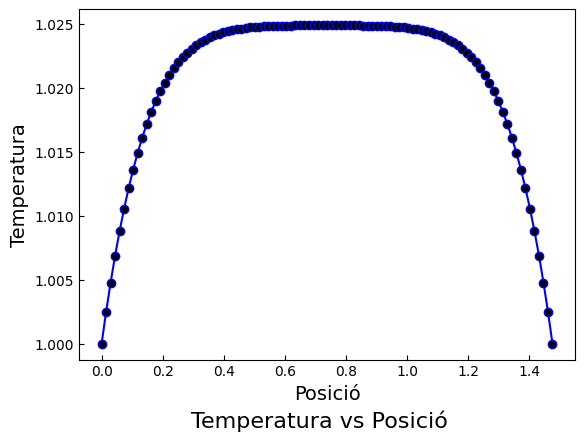
\includegraphics[width=\textwidth]{images/T_vs_z_at2.png}
        \caption{} 
        \label{fig:err_euler_imp_at2}
    \end{subfigure}
    \caption{Error numèric del mètode d'Euler implícit respecte a la solució analítica pel mallat 1.0 (a) i 0.5 (b) a $\tilde{t}=0.025$ fent servir el mètode d'Euler implícit.}
    \label{fig:err_euler_implicit}
\end{figure}
\subsection{Crank-Nicolson}
Fem servir ara l'esquema de Crank-Nicholson per a resoldre l'equació \eqref{EDP_norm}. Tornant a discretitzar la derivada temporal per la dreta i fent una mitjana de la segonda derivada entre $i$ i $(i+1)$ obtenim la relació de recurrència
\begin{equation*}
    -\gamma\tilde{T}_{j+1}^{i+1} + (2+2\gamma)\tilde{T}_{j}^{i+1} - \gamma \tilde{T}_{j-1}^{i+1} = \gamma \tilde{T}_{j+1}^{i} + (2-2\gamma)\tilde{T}_{j}^{i} + \gamma \tilde{T}_{j-1}^{i} - 2\Delta t
\end{equation*}
Podem escriure cada banda de la igualtat en forma matricial, obtenint
\begin{equation*}
    \vec{a} + \mathbb{A} \vec{T}_{i+1} = \vec{b} + \mathbb{B}\vec{T}_{i} \hspace{4 mm} \Rightarrow \hspace{4 mm} \vec{T}_{i+1} = \mathbb{A}^{-1}(\vec{c}+\mathbb{B}\vec{T}_{i})
\end{equation*}
on definim els vectors $\vec{T}_{i}$ i $\vec{T}_{i+1}$ de la mateixa manera que al aplicar Euler implícit i on definim
\begin{equation*}
    \vec{a} = \begin{matrix} (-\gamma T_c & 0 & \dots & 0 & -\gamma T_c)^{\text{t}}\end{matrix} \hspace{4 mm} \text{,} \hspace{4 mm} \vec{b} = \begin{matrix} (\gamma T_c + 2\Delta t & 2\Delta t & \dots & 2\Delta t & \gamma T_c + 2\Delta t)^{\text{t}} \end{matrix} \hspace{4 mm} \text{,} \hspace{4 mm} \vec{c} = \vec{b} - \vec{a}
\end{equation*}
\begin{equation*}
    \mathbb{A} = \text{tridiag}(-\gamma,2+2\gamma,-\gamma) \hspace{4 mm} \text{,} \hspace{4 mm} \mathbb{B} = \text{tridiag}(\gamma,2-2\gamma,\gamma)
\end{equation*}
Aplicant les respectives iteracions obtenim els plots de la Fig. \ref{fig:crank_nicholson} i Fig. \ref{err_crank_nicholson}
\begin{figure}[h]
    \centering
    \begin{subfigure}[b]{0.35\textwidth}
        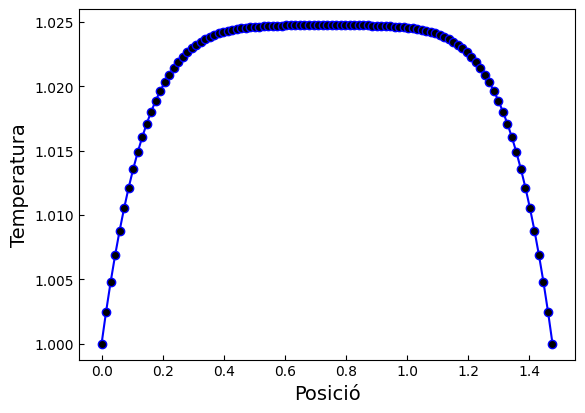
\includegraphics[width=\textwidth]{images/T_vs_z_CN_at1.png} 
        \caption{}
        \label{fig:CN_at1}
    \end{subfigure}
    \hspace{1.5cm}
    \begin{subfigure}[b]{0.35\textwidth}
        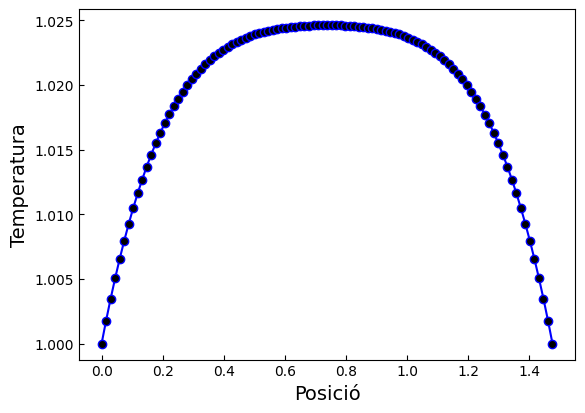
\includegraphics[width=\textwidth]{images/T_vs_z_CN_at2.png}
        \caption{} 
        \label{fig:CN_at2}
    \end{subfigure}
    \caption{Solució numèrica pel mallat 1.0 (a) i 0.5 (b) a $\tilde{t}=0.025$ fent servir el mètode de Crank-Nicholson.}
    \label{fig:crank_nicholson}
\end{figure}
\begin{figure}[h]
    \centering
    \begin{subfigure}[b]{0.35\textwidth}
        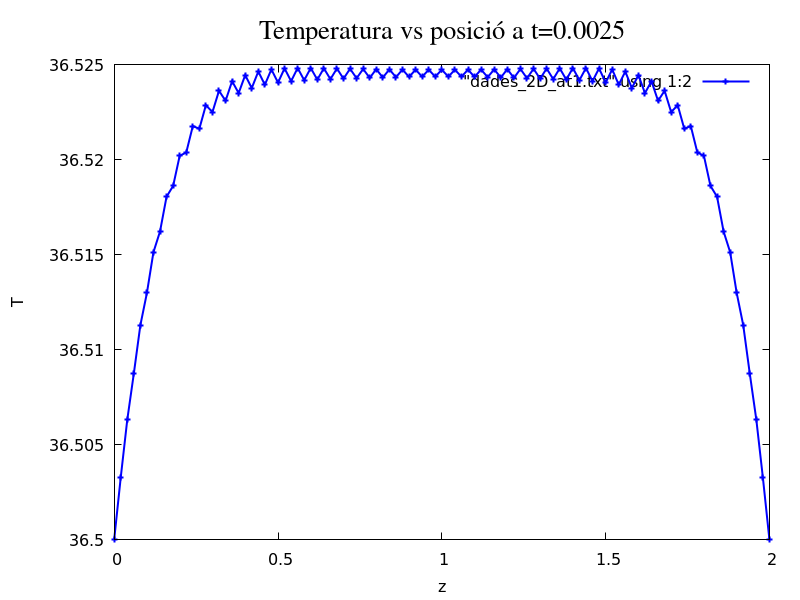
\includegraphics[width=\textwidth]{images/T_vs_z_at1.png} 
        \caption{}
        \label{fig:err_CN_at1}
    \end{subfigure}
    \hspace{1.5cm}
    \begin{subfigure}[b]{0.35\textwidth}
        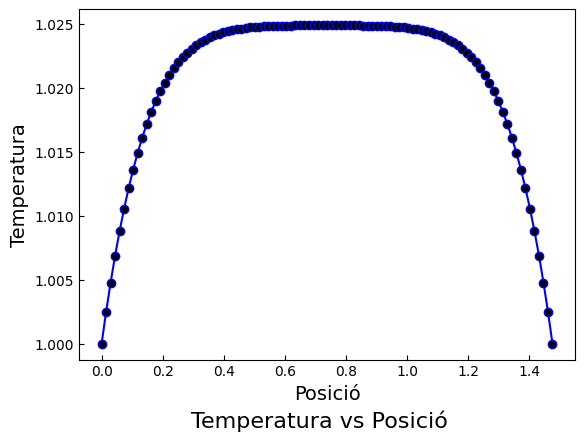
\includegraphics[width=\textwidth]{images/T_vs_z_at2.png}
        \caption{} 
        \label{fig:err_CN_at2}
    \end{subfigure}
    \caption{Error respecte a la solució analítica pel mallat 0.51 (a) i 0.25 (b) a $\tilde{t}=0.025$ fent servir el mètode de Crank-Nicholson.}
    \label{fig:crank_nicholson}
\end{figure}

\section{Solució del problema d'IVS}
Per determinar el temps necessari hem d'aplicar la senyal elèctrica per tractar eficientment al pacient, farem servir Crank-Nicolson per solucionar l'equació de difusió. Amb aquest mètode, anem trobant iterativament la distribució de temperatura per a un temps creixent. En cada iteració avaluem les temperatures cercant el tractament més eficient possible. Per aconseguir això, a cada distribució de temperatura per una mateixa posició temporal imposem diverses condicions. \\ Primerament que en cap posició espacial pel temps t s'arribi a una temperatura superior o igual a 80ºC. Segonament, que cap part de la regió sana (per $x\in(0,0.75) \cup (1.25,2)$ en cm) arribi o superi els 50ºC. Imposant aquestes dues condicions iterativament arribem a un temps màxim en el qual es compleixen. Amb aquest temps, ens assegurem que per aquest i temps menors el tractament no serà perillós pel pacient. Ara, cerquem que la màxima regió de teixit malalt estigui entre 50ºC i 80ºC. Com hem imposat que en la frontera entre teixits ($x =0.75cm$ i $x=1.25cm$) s'arribes a la temperatura màxima però inferior a 50ºC, tot el teixit malalt es trobara a una temperatura superior. Llavors, la regió més externa del teixit malalt arriba com a mínim a 50ºC en el temps màxim que hem trobat. Això es pot comprovar en la figura \ref{fig:solucion_ivs}, on en vermell es mostra la frontera entre el teixit malalt i el saludable. La figura mostra la distribució de la temperatura pel temps $t =  63.17$ que es la nostra proposta com a temps més eficient i que compleix les condicions imposades. Entre les franjes vermelles es troba el teixit malalt, que podem comprovar que es trobara per damunt de 50ºC, i per fora de les franjes s'observa el teixit saludable que no supera els 50ºC.

\begin{figure}[h]
    \centering
    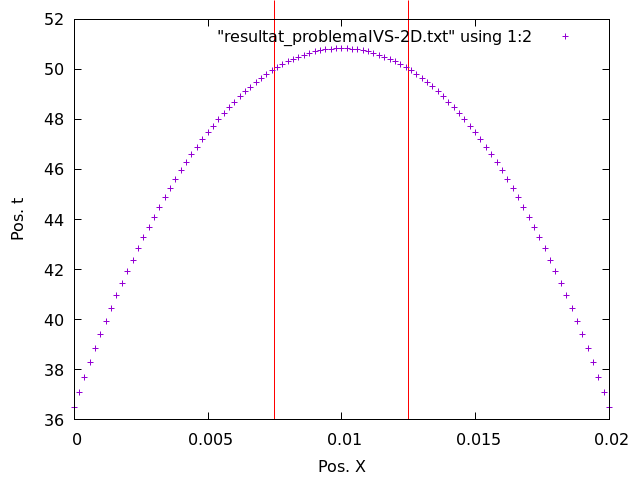
\includegraphics[width=0.5\linewidth]{images/solucion_IVS-2D.png}
    \caption{Distribució de temperatura per al temps màxim trobat de 63.17 segons}
    \label{fig:solucion_ivs}
\end{figure}

\section{Conclusions}
En esta práctica, hemos modelado el proceso de ablación cardíaca IVS para evaluar su eficacia y %
seguridad utilizando diferentes métodos numéricos. A partir de la solución analítica de la ecuación de difusión de calor y las simulaciones numéricas implementadas con métodos explícitos, implícitos y de Crank-Nicolson, se logró determinar el tiempo óptimo de aplicación del tratamiento eléctrico que satisface las condiciones de seguridad requeridas: mantener el tejido sano por debajo de los 50 ºC, evitar que cualquier punto alcance los 80 ºC, y asegurar que la mayor parte del tejido enfermo permanezca entre los 50 ºC y los 80 ºC.

Los resultados numéricos muestran que el método de Crank-Nicolson ofrece un equilibrio óptimo entre precisión y estabilidad, superando las limitaciones de los métodos explícito e implícito en cuanto a oscilaciones o sobrecostos computacionales. De este modo, se determinó que el tiempo ideal para este procedimiento es de 192.78 segundos, garantizando un tratamiento eficiente y seguro.

Finalmente, esta práctica demuestra la utilidad de las técnicas de modelado y simulación numérica en contextos médicos, brindando herramientas para mejorar la comprensión y la implementación de procedimientos clínicos.

\section{Annex}\label{Annex I}
\subsection{Solució analítica}
Per a una equació diferencial del tipus
\begin{equation*}
    \frac{\partial f(x,t)}{\partial t} = \frac{\partial^2 f(x,t)}{\partial x^2} + q(x,t)
\end{equation*}
amb les condicions inicials i de contorn: $f(x,0) = \beta$, $f(0,t)=f(t,1)= \beta$. Sigin $x=0$ i $x=1$ les fronteres del sistema, tenim la solució
\begin{equation*}
    f(x,t) = \beta +\sum_{n=1}^{\infty} b_n(t) = \left( \frac{1-e^{-n^2\pi^2t}}{n^2\pi^2}\right)\sin{(n\pi x)}
\end{equation*}
on es defineix
\begin{equation*}
    b_n(t) = 2\int_{0}^{1} q(x,t)\sin{(n\pi x)}\text{d}x
\end{equation*}
\bibliographystyle{plain} 
\bibliography{referencies.bib}
\end{document}